\documentclass[aspectratio=169]{beamer}

\usetheme{Madrid}
\usecolortheme{default}
\usepackage[utf8]{inputenc}
\usepackage[T1]{fontenc}
\usepackage{amsmath}
\usepackage{amssymb}
\usepackage{xcolor}
\usepackage{mdframed}
\usepackage{tikz}
\usepackage{amsmath}
\usetikzlibrary{arrows.meta, positioning, shapes.geometric, calc}

% Farben
\definecolor{tugreen}{RGB}{0, 110, 80}
\definecolor{alertred}{RGB}{180, 0, 0}
\definecolor{extramethod}{RGB}{180, 80, 0}

\setbeamercolor{structure}{fg=tugreen}
\setbeamercolor{frametitle}{bg=tugreen, fg=white}
\setbeamercolor{title}{bg=tugreen, fg=white}

% Titelseite
\title[DRAUSP als RL-Problem]{Modellierung des DRAUSP-Problems\\als Reinforcement-Learning-Problem}
\subtitle{DQN, Action Masking, Monotonicity-aware DQN}
\author{Niklas Fritz, Felix Fritz}
\date{21.05.2026}

% -----------------------------------------------------------------------
\begin{document}
% -----------------------------------------------------------------------

\begin{frame}
  \titlepage
\end{frame}

% -----------------------------------------------------------------------
\begin{frame}{Gliederung}
  \tableofcontents
\end{frame}

% -----------------------------------------------------------------------
\section{Das DRAUSP-Problem}
% -----------------------------------------------------------------------

\begin{frame}{Das DRAUSP-Problem}

  \textbf{Dynamic Resource Allocation Under Stochastic Prices (DRAUSP)}

  \begin{block}{Problemstellung}
    Gegeben: Serviceperiode mit $K$ Zeitslots der Kapazität $C_k$, $T_d$ Anfragen, die sequenziell eintreffen. Jede Anfrage $i$ hat:
    \begin{itemize}
      \item einen \textbf{Erlös} $r_i \in \mathbb{R}$
      \item einen \textbf{Kapazitätsbedarf} $q_i \in \mathbb{N}^K$ über $K$ Zeitslots
    \end{itemize}
  \end{block}

  \bigskip
  \begin{block}{Entscheidung}
    Für jede Anfrage muss \textbf{sofort und unwiderruflich} entschieden werden:
    \begin{itemize}
      \item \textbf{Ablehnen} $\rightarrow$ Erlös $= 0$
      \item \textbf{Akzeptieren ab Slot $k$} $\rightarrow$ Erlös $= r_i$, Kapazitäten werden reduziert
    \end{itemize}
  \end{block}

  \textbf{Ziel:} Maximiere \textbf{Gesamterlöses} unter Einhaltung der Kapazitätsschranken $C_k$.

\end{frame}

% -----------------------------------------------------------------------
\section{Grundlagen: Reinforcement Learning}
% -----------------------------------------------------------------------
\begin{frame}{Reinforcement Learning -- Grundprinzip}
  \begin{columns}
    \column{0.5\textwidth}
     \begin{block}{Kernidee}
        Ein \textbf{Agent} interagiert mit einer \textbf{Umgebung} und lernt durch
        Versuch und Irrtum eine optimale \textbf{Policy} $\pi$.
      \end{block}

    \column{0.5\textwidth}
      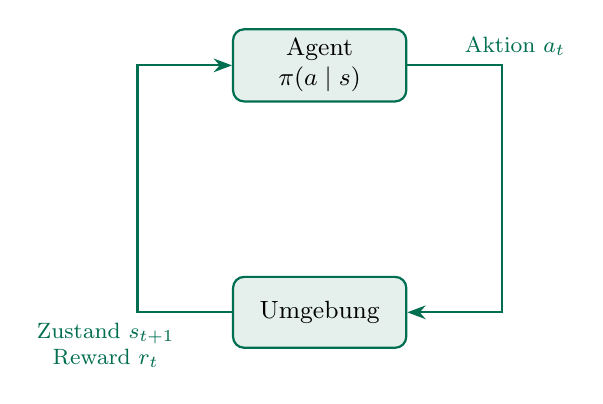
\begin{tikzpicture}[
        node distance=1.8cm,
        box/.style={rectangle, draw=tugreen, thick, rounded corners,
                    minimum width=2.2cm, minimum height=0.9cm,
                    fill=tugreen!10, align=center, font=\small},
        arr/.style={-{Stealth}, thick, tugreen}
      ]
        \node[box] (agent) {Agent\\$\pi(a\mid s)$};
        \node[box, below=2.2cm of agent] (env) {Umgebung};

        \draw[arr] (agent.east) -- ++(1.2,0)
              node[midway, above right, font=\footnotesize]{Aktion $a_t$}
              |- (env.east);

        \draw[arr] (env.west) -- ++(-1.2,0)
              node[midway, below left, align=center, font=\footnotesize]{Zustand $s_{t+1}$\\Reward $r_t$}
              |- (agent.west);
      \end{tikzpicture}
  \end{columns}

\end{frame}

\begin{frame}{Reinforcement Learning -- Grundprinzip}

  \begin{columns}
    \column{0.5\textwidth}
      \textbf{Zentrale Komponenten:}
      \begin{itemize}
        \item \textbf{Zustand} $s \in \mathcal{S}$
        \item \textbf{Aktion} $a \in \mathcal{A}$
        \item \textbf{Reward} $r: S \times A \to P(\mathbb{R})$
        \item \textbf{Policy} $\pi(a \mid s): S \to P(A)$
        \item goal: \textbf{Maximiere den erwarteten kumulierten Reward}
         \begin{equation*}
      \pi^* =\arg\max_{\pi} \mathbb{E}_{\pi}\Bigg[\sum_{t=1}^{\infty}\gamma^{t} r_t\Bigg]
         \end{equation*}
      \end{itemize}

    \column{0.5\textwidth}
      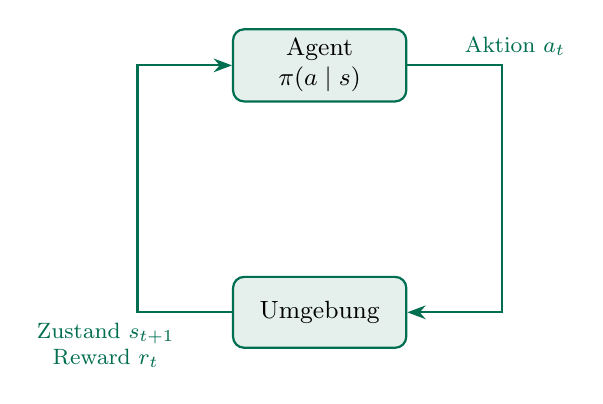
\begin{tikzpicture}[
        node distance=1.8cm,
        box/.style={rectangle, draw=tugreen, thick, rounded corners,
                    minimum width=2.2cm, minimum height=0.9cm,
                    fill=tugreen!10, align=center, font=\small},
        arr/.style={-{Stealth}, thick, tugreen}
      ]
        \node[box] (agent) {Agent\\$\pi(a\mid s)$};
        \node[box, below=2.2cm of agent] (env) {Umgebung};

        \draw[arr] (agent.east) -- ++(1.2,0)
              node[midway, above right, font=\footnotesize]{Aktion $a_t$}
              |- (env.east);

        \draw[arr] (env.west) -- ++(-1.2,0)
              node[midway, below left, align=center, font=\footnotesize]{Zustand $s_{t+1}$\\Reward $r_t$}
              |- (agent.west);
      \end{tikzpicture}
  \end{columns}

\end{frame}

% -----------------------------------------------------------------------
\begin{frame}{Q-Learning -- Policy aus Q-Werten}

  \begin{block}{Q-Funktion}
    $Q(s, a)$ gibt den erwarteten kumulierten Reward an, wenn man in Zustand $s$ die Aktion $a$ wählt.
  \end{block}

  \bigskip
  \begin{columns}[T]
    \column{0.55\textwidth}
      \textbf{Optimale Policy:}
      \[
        \pi^*(s) \;=\; \arg\max_{a \in \mathcal{A}}\; Q^*(s, a)
      \]
      Der Agent wählt stets die Aktion mit dem \textbf{höchsten Q-Wert}.

      \bigskip
      \textbf{Lernregel (Bellman):}
      \[
        Q(s,a) \;\leftarrow\; r + \gamma \cdot \max_{a'} Q(s', a')
      \]
      \begin{itemize}
        \item $\gamma \in [0,1]$: Diskontierungsfaktor
        \item $r$: unmittelbarer Reward
        \item $\max_{a'} Q(s', a')$: bester zukünftiger Wert
      \end{itemize}

    \column{0.45\textwidth}
      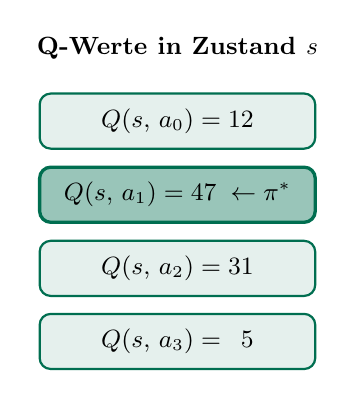
\begin{tikzpicture}[
        node distance=0.5cm,
        box/.style={rectangle, draw=tugreen, thick, rounded corners,
                    minimum width=3.5cm, minimum height=0.7cm,
                    fill=tugreen!10, align=center, font=\small},
        best/.style={rectangle, draw=tugreen, very thick, rounded corners,
                    minimum width=3.5cm, minimum height=0.7cm,
                    fill=tugreen!40, align=center, font=\small\bfseries}
      ]
        \node[font=\small\bfseries] (title) {Q-Werte in Zustand $s$};
        \node[box,  below=0.3cm of title] (a0) {$Q(s,\, a_0) = 12$};
        \node[best, below=0.2cm of a0]   (a1) {$Q(s,\, a_1) = 47 \;\leftarrow \pi^*$};
        \node[box,  below=0.2cm of a1]   (a2) {$Q(s,\, a_2) = 31$};
        \node[box,  below=0.2cm of a2]   (a3) {$Q(s,\, a_3) = \phantom{0}5$};
      \end{tikzpicture}
  \end{columns}

\end{frame}

\begin{frame}{Deep Q-Network (DQN)}

  \begin{block}{Warum ein neuronales Netz?}
    Zustandsraum zu groß, um $Q(s,a)$ tabellarisch zu speichern ($Q \in \mathbb{R}^{\vert S \vert \times \vert A \vert}$)
    $\rightarrow$ ein \textbf{neuronales Netz} approximiert $Q(s,a)$ für alle Aktionen gleichzeitig.
  \end{block}

  \bigskip
  \begin{mdframed}[backgroundcolor=gray!20, , hidealllines=true]
    $$
      Q(\cdot \vert \theta_{DQN}): \quad s \xrightarrow{\text{DQN}}   \begin{pmatrix} Q(s, a_1) \\ Q(s, a_2) \\ \vdots \\ Q(s, a_N) \end{pmatrix}
    $$
\end{mdframed}

\end{frame}
% -----------------------------------------------------------------------
\begin{frame}{Deep Q-Network (DQN)}
  \textbf{Training des DQN:}
  \begin{itemize}
    \item \textbf{Replay Buffer}: Erfahrungen $(s, a, r, s')$ werden gespeichert und zufällig
          gesampelt
    \item \textbf{Loss-Funktion}: \textbf{MSE} zwischen Zielwert $y_i$ und Vorhersage $Q(s_i, a_i; \theta^{DQN})$
  \begin{mdframed}[backgroundcolor=gray!20, , hidealllines=true]
    \begin{equation*}
        \begin{split}
             &L(\theta^{DQN}) = \frac{1}{N} \sum_{i} (y_i - Q(s_i, a_i; \theta^{DQN}))^2, \\
            &\theta^{DQN} \leftarrow \theta^{DQN} - \alpha \nabla_{\theta^{DQN}} L(\theta^{DQN})
        \end{split}
  \end{equation*}
  \end{mdframed} 
    \item \textbf{Target-Netz}: zweites, seltener aktualisiertes Netz stabilisiert das Training
    \item \textbf{$\varepsilon$-Greedy}: Balance zwischen Exploration und Exploitation
    \item \textbf{Gradient Clipping}: verhindert explodierende Gradienten
  \end{itemize}

\end{frame}
% -----------------------------------------------------------------------
\section{Modellierung als RL-Problem}
% -----------------------------------------------------------------------

\begin{frame}{Zustandsraum}

  \begin{block}{Zustandsvektor $s \in \mathcal{S} \subseteq \mathbb{R}^{2K+2}$}
    \[
      s \;=\; \bigl(t,\;\hat{C}_1,\;\ldots,\;\hat{C}_K,\;r,\;q_1,\;\ldots,\;q_K\bigr)
    \]
  \end{block}

  \bigskip
  \begin{tabular}{lll}
    \hline
    \textbf{Komponente} & \textbf{Bedeutung} & \textbf{Wertebereich} \\
    \hline
    $t$ & aktueller Zeitschritt & $\{1, \ldots, T_d\}$ \\
    $\hat{C}_k$ & verbleibende Kapazität in Slot $k$ & $\{0, \ldots, C_k\}$ \\
    $r$ & Erlös der aktuellen Anfrage & $\mathbb{R}_{\geq 0}$ \\
    $q_k$ & benötigter Bedarf in Slot $k$ & $\{0, \ldots, C_k\}$ \\
    \hline
  \end{tabular}

  \bigskip
  \textbf{Initialzustand:}
  \[
    s_1 = \bigl(1,\;C_1,\;\ldots,\;C_K,\;r_1,\;q_1^1,\;\ldots,\;q_1^K\bigr)
  \]

\end{frame}

% -----------------------------------------------------------------------
\begin{frame}{Aktionsraum und Übergangsfunktion}

  \begin{block}{Aktionsraum $\mathcal{A} = \{0, 1, \ldots, K\}$}
    \begin{itemize}
      \item \textbf{Aktion $0$:} Anfrage ablehnen $\rightarrow$ Kapazitäten unverändert
      \item \textbf{Aktion $k > 0$:} Anfrage ab Slot $k$ einplanen
            $\rightarrow$ $\hat{C}_{k+i} \leftarrow \hat{C}_{k+i} - q_i$ für $i = 0, \ldots, \ell_q - 1$
    \end{itemize}
  \end{block}

  \bigskip
  \begin{block}{Reward-Funktion}
    \[
      R(s, a) =
      \begin{cases}
        r    & \text{Akzeptieren, Kapazität ausreichend} \\
        0    & \text{Ablehnen} \\
        -100 & \text{ungültige Aktion (Kapazitätsverletzung)}
      \end{cases}
    \]
  \end{block}

  \bigskip
  \textbf{Episode endet} (\texttt{terminated} $=$ True), wenn:
  \begin{itemize}
    \item alle $T_d$ Anfragen abgearbeitet wurden, \textbf{oder}
    \item eine ungültige Aktion gewählt wurde
  \end{itemize}

\end{frame}

% -----------------------------------------------------------------------
\section{Das Problem der ungültigen Aktionen}
% -----------------------------------------------------------------------

\begin{frame}{Das Problem der ungültigen Aktionen}

  \begin{alertblock}{Problem}
    Nicht jede Aktion $a \in \mathcal{A}$ ist in jedem Zustand \textbf{zulässig}!
  \end{alertblock}

  \bigskip
  \textbf{Zwei Arten von ungültigen Aktionen:}

  \begin{enumerate}
    \item \textbf{Slot zu weit rechts:} \quad $\ell_q + a - 1 > K$ \\
          {\small Die Anfrage würde über den letzten Slot hinausragen.}

    \bigskip
    \item \textbf{Kapazitätsverletzung:} \quad $\exists\, i:\; \hat{C}_{a+i} < q_i$ \\
          {\small Die verbleibende Kapazität reicht nicht aus.}
  \end{enumerate}

  \bigskip
  \begin{block}{Konsequenz für Standard-DQN}
    Ein Standard-DQN ohne Behandlung ungültiger Aktionen wählt per $\arg\max$ ggf.
    eine unzulässige Aktion $\rightarrow$ Reward $= -100$ $\rightarrow$
    \textbf{instabiles, langsames Training}.
  \end{block}

\end{frame}

% -----------------------------------------------------------------------
\begin{frame}{Action Masking -- Lösung}

  \begin{block}{Idee}
    Ungültige Aktionen erhalten \textbf{vor der Auswahl} einen Q-Wert von $-\infty$,
    sodass $\arg\max$ sie niemals wählt.
  \end{block}

  \bigskip
  \textbf{Action Masking im Policy und Target-Netz:}

  \begin{columns}
    \column{0.5\textwidth}
      \begin{exampleblock}{1. Aktionsauswahl}
        \[
          \tilde{Q}(s,a) =
          \begin{cases}
            Q_\pi(s,a) & a \in \mathcal{A}_{\text{valid}}(s) \\
            -\infty    & \text{sonst}
          \end{cases}
        \]
        \[
          a^* = \arg\max_{a}\, \tilde{Q}(s,a)
        \]
      \end{exampleblock}
  \end{columns}
  \bigskip
  Außerdem samplet man im $\epsilon$-Greedy-Verfahren nur aus den gültigen Aktionen $\mathcal{A}_{\text{valid}}(s)$.
\end{frame}

% -----------------------------------------------------------------------
\section{Gymnasium-Implementierung}
% -----------------------------------------------------------------------

\begin{frame}{Gymnasium-Umgebung -- Interface}

  \begin{block}{Gymnasium}
    Standardisiertes Python-Interface für RL-Umgebungen --
    kompatibel mit gängigen RL-Bibliotheken.
  \end{block}

  \bigskip
  \textbf{Pflichtmethoden (Gymnasium-Standard):}

  \medskip
  \begin{tabular}{lll}
    \hline
    \textbf{Methode} & \textbf{Rückgabe} & \textbf{Bedeutung} \\
    \hline
    \texttt{reset()} & \texttt{obs, info} & Neue Episode starten \\
    \texttt{step(action)} & \texttt{obs, r, terminated, truncated, info} & Schritt ausführen \\
    \texttt{render()} & -- & Zustand visualisieren \\
    \hline
  \end{tabular}

  \medskip
  \textcolor{extramethod}{\textbf{Eigene Erweiterung für Action Masking:}}\\[0.3em]
  \textcolor{extramethod}{\texttt{get\_valid\_actions()} $\;\rightarrow\;$ \texttt{list[int]}}
  \quad {\small Gibt alle zulässigen Aktionen im aktuellen Zustand zurück.}

\end{frame}

% -----------------------------------------------------------------------
\section{Zusammenfassung \& Ausblick}
% -----------------------------------------------------------------------

\begin{frame}{Zusammenfassung}

  \begin{block}{Beitrag}
    Modellierung des DRAUSP-Problems als Reinforcement-Learning-Problem
    mit einer standardisierten Gymnasium-Umgebung.
  \end{block}
  \bigskip
  \textbf{Geplanter Vergleich:}

  \medskip
  \begin{tabular}{lll}
    \hline
    \textbf{Methode} & \textbf{Typ} & \textbf{Action Masking} \\
    \hline
    Random Policy        & Baseline         & {--} \\
    DQN ohne Masking     & RL               & \textcolor{alertred}{nein} \\
    DQN mit Masking      & RL               & \textcolor{tugreen}{ja} \\
    Monotones DQN        & RL (Erweiterung) & \textcolor{tugreen}{ja} \\
    \hline
  \end{tabular}

\end{frame}

% -----------------------------------------------------------------------
\begin{frame}{Ausblick}

  \begin{enumerate}

    \item \textbf{Allgemeiner Aktionsraum} \\
          Bisher: feste Requestgröße $\ell_q$.
          Geplant: variable Requestgrößen

    \bigskip
    \item \textbf{Monotone Neural Networks} \\
          Architektur erzwingt strukturelle Monotonie in Kapazitäten und Erlös:
          \[
            \hat{C}_k \uparrow \;\Rightarrow\; Q(s,a) \uparrow
            \qquad\qquad
            r \uparrow \;\Rightarrow\; Q(s,a) \uparrow
          \]

    \bigskip
    \item \textbf{Evaluation auf Benchmark-Instanzen} \\
          \begin{itemize}
            \item \textbf{Konvergenzgeschwindigkeit}: Anzahl Episoden bis zur Stabilisierung
            \item \textbf{Trainings-Stabilität}: Varianz des kumulierten Rewards (Sample-Varianz)
            \item \textbf{Generalisierung}: Out-of-sample Performance auf ungesehenen Instanzen
          \end{itemize}

    \bigskip
    \item \textbf{Hyperparameter-Analyse} \\
          Exploration-Faktor $\epsilon$, Diskontierungsfaktor $\gamma$, Replay-Buffer-Größe, Netzwerkarchitektur

  \end{enumerate}

\end{frame}

% -----------------------------------------------------------------------
\begin{frame}
  \begin{center}
    \Huge\textbf{Vielen Dank!}\\[1em]
    \large Fragen?
  \end{center}
\end{frame}

\end{document}